\section{Классификация точек покоя}

	В данном разделе рассмотрим классификацию точек покоя для двумерных вещественных стационарных нелинейных систем обыкновенных дифференциальных уравнений первого порядка:
	\[ \vec{\dot{x}} = \vec{f}\pares{\vec{x}}, ~ \vec{x} = \begin{pmatrix} x_1 \\ x_2 \end{pmatrix} \]

	Для данной системы в окрестности точки покоя $\vec{x} = \vec{x}_0$ будем рассматривать систему первого приближения:
	\[ \vec{\dot{x}} = A \cdot \vec{x}, \]
	где $A = \tilde{J}\pares{\vec{x}} \sat_{\vec{x} = \vec{x}_0}$ -- матрица Якоби в точке покоя, двумерная матрица постоянных коэффициентов. Положим, что матрица $A$ -- разложима с помощью матрицы преобразований $P$, и верхнетреугольной жордановой формы $J$: $A = PJP^{-1}$. Следующая классификация будет рассмотрена для систем вида $\vec{\dot{x}} = J \vec{x}$. Для построения фазового пространства конкретных систем, необходимо построить матрицу преобразований $P$, и по представленным ниже правилам применить матрицу $P$ как матрицу аффинного преобразования системы координат.

	Пусть у матрицы $J$ собственные значения $\lambda_1$ и $\lambda_2$. Собственные вектора $\vec{v}_1, \vec{v}_2$ матрицы $A$ представляют собой соответствующие собственным значениям $\lambda_1, \lambda_2$ столбцы матрицы преобразований $P$. Будем полагать, что собственные вектора рассматриваемой системы равны соответственно $\vec{v}_1 = \begin{pmatrix} 1 \\ 0 \end{pmatrix}$ и $\vec{v}_2 = \begin{pmatrix} 0 \\ 1 \end{pmatrix}$, и соответствующие им прямые на изображениях будут отражены красными линиями. Тогда введем классификацию точек покоя:
	\begin{enumerate}
		\item \textit{Невырожденный узел} -- случай, когда ненулевые вещественные собственные значения $\lambda_{1, 2}$ не равны между собой, и одного знака (положим $\abs{\lambda_1} < \abs{\lambda_2}, ~ \lambda_{1, 2} \in \mathbb{R}, ~ \lambda_{1, 2} \neq 0$). Интегральные кривые на фазовой плоскости сходятся в (в случае отрицательных собственных значений), или исходят из (в случае положительных собственных значений) точки покоя, и изгибаются по направлению прямой, построенной на основе собственного вектора с наименьшим по модулю собственным значением (от прямой с направляющим вектором $\vec{v}_2$ к прямой с направляющим вектором $\vec{v}_1$). На изображениях ниже рассмотрены случаи $J = \begin{pmatrix} -1 & 0 \\ 0 & -2 \end{pmatrix}$ (устойчивый невырожденный узел, рис. \ref{Stability:StableKnot}) и $J = \begin{pmatrix} 2 & 0 \\ 0 & 3 \end{pmatrix}$ (неустойчивый невырожденный узел, рис. \ref{Stability:UnstableKnot}).

			\begin{multicols}{2}

				\begin{figure}[H]
					\centering
					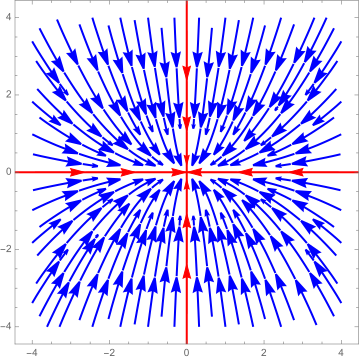
\includegraphics[width=0.4\textwidth]{additional/Stability/Points/StableKnot.pdf}
					\caption{Устойчивый невырожденный узел}
					\label{Stability:StableKnot}
				\end{figure}

			\columnbreak

				\begin{figure}[H]
					\centering
					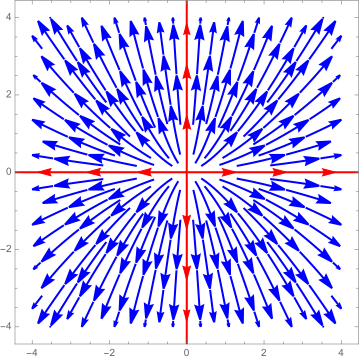
\includegraphics[width=0.4\textwidth]{additional/Stability/Points/UnstableKnot.pdf}
					\caption{Неустойчивый невырожденный узел}
					\label{Stability:UnstableKnot}
				\end{figure}

			\end{multicols}

		\item \textit{Вырожденный узел} -- случай, когда ненулевые вещественные собственные значения $\lambda_{1, 2}$ равны между собой, при этом линейно-зависимы (положим $\lambda_1 = \lambda_2 = \lambda \neq 0, ~ \lambda \in \mathbb{R}$). Интегральные кривые на фазовой плоскости сходятся в (в случае отрицательных собственных значений), или исходят из (в случае положительных собственных значений) точки покоя, и вращаются в направлении, обратном положительному направлению вращения системы координат (против часовой стрелки). На изображениях ниже рассмотрены случаи $J = \begin{pmatrix} -2 & 1 \\ 0 & -2 \end{pmatrix}$ (устойчивый вырожденный узел, рис. \ref{Stability:StableDegKnot}) и $J = \begin{pmatrix} 3 & 1 \\ 0 & 3 \end{pmatrix}$ (неустойчивый вырожденный узел, рис. \ref{Stability:UnstableDegKnot}).

			\begin{multicols}{2}

				\begin{figure}[H]
					\centering
					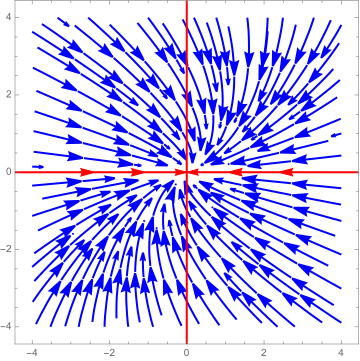
\includegraphics[width=0.4\textwidth]{additional/Stability/Points/StableDegKnot.pdf}
					\caption{Устойчивый вырожденный узел}
					\label{Stability:StableDegKnot}
				\end{figure}

			\columnbreak

				\begin{figure}[H]
					\centering
					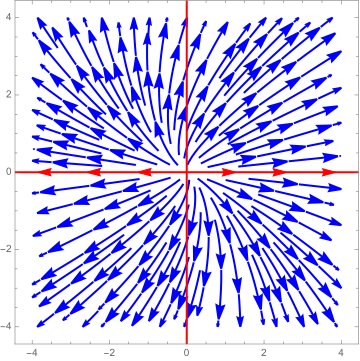
\includegraphics[width=0.4\textwidth]{additional/Stability/Points/UnstableDegKnot.pdf}
					\caption{Неустойчивый вырожденный узел}
					\label{Stability:UnstableDegKnot}
				\end{figure}

			\end{multicols}

		\item \textit{Дикритический узел} -- случай, когда ненулевые вещественные собственные значения $\lambda_{1, 2}$ равны между собой, при этом линейно-независимы (положим $\lambda_1 = \lambda_2 = \lambda \neq 0, ~ \lambda \in \mathbb{R}$). Интегральные кривые на фазовой плоскости сходятся в (в случае отрицательных собственных значений), или исходят из (в случае положительных собственных значений) точки покоя, и представляют собой прямые линии. На изображениях ниже рассмотрены случаи $J = \begin{pmatrix} -1 & 0 \\ 0 & -1 \end{pmatrix}$ (устойчивый дикритический узел, рис. \ref{Stability:StableDicritKnot}) и $J = \begin{pmatrix} 2 & 0 \\ 0 & 2 \end{pmatrix}$ (неустойчивый дикритический узел, рис. \ref{Stability:UnstableDicritKnot}).

			\begin{multicols}{2}

				\begin{figure}[H]
					\centering
					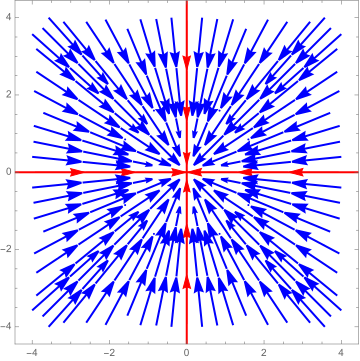
\includegraphics[width=0.4\textwidth]{additional/Stability/Points/StableDicritKnot.pdf}
					\caption{Устойчивый дикритический узел}
					\label{Stability:StableDicritKnot}
				\end{figure}

			\columnbreak

				\begin{figure}[H]
					\centering
					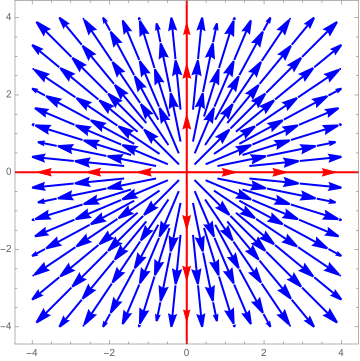
\includegraphics[width=0.4\textwidth]{additional/Stability/Points/UnstableDicritKnot.pdf}
					\caption{Неустойчивый дикритический узел}
					\label{Stability:UnstableDicritKnot}
				\end{figure}

			\end{multicols}

		\item \textit{Седло} -- случай, когда ненулевые вещественные собственные значения $\lambda_{1, 2}$ имеют противоположные знаки (положим $\lambda_1 < 0 < \lambda_2, ~ \lambda_{1, 2} \in \mathbb{R}$). Интегральные кривые на фазовой плоскости представляют собой семейство гипербол в окрестности точки покоя. Направление задается от прямой, построенной на основе собственного вектора с положительным собственным значением в сторону прямой, построенной на основе собственного вектора с отрицательным собственным значением. Седловая точка является неустойчивой. На изображении ниже рассмотрен случай $J = \begin{pmatrix} -1 & 0 \\ 0 & 2 \end{pmatrix}$ (седловая точка, рис. \ref{Stability:Saddle}).

			\begin{figure}[H]
				\centering
				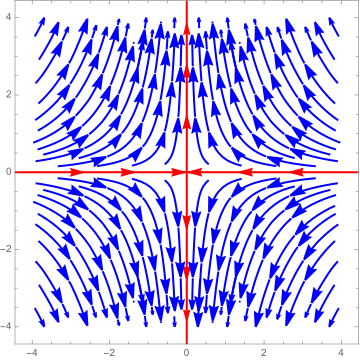
\includegraphics[width=0.4\textwidth]{additional/Stability/Points/Saddle.pdf}
				\caption{Неустойчивая седловая точка}
				\label{Stability:Saddle}
			\end{figure}

		\item \textit{Фокус} -- случай, когда комплексно-сопряженные собственные значения $\lambda_{1, 2}$ имеют ненулевую вещественную часть (положим $\lambda_{1, 2} = \alpha \pm i \beta, ~ \alpha, \beta \in \mathbb{R}, ~ \lambda_{1, 2} \in \mathbb{C}$). Интегральные кривые представляют собой вращающийся поток, сходящийся к (в случае отрицательной вещественной части собственных значений), или исходящихся от (в случае положительной вещественной части собственных значений) точки покоя (при этом ее не касается). Вращение производится в положительном направлении вращения системы координат (по часовой стрелке) в случае, если вещественная жорданова форма является обобщением комплексного числа. На изображениях ниже рассмотрены случаи $J = \begin{pmatrix} -1 & -2 \\ 2 & -1 \end{pmatrix}$ (устойчивый фокус, рис. \ref{Stability:StableFocal}) и $J = \begin{pmatrix} 2 & -1 \\ 1 & 2 \end{pmatrix}$ (неустойчивый фокус, рис. \ref{Stability:UnstableFocal}).

			\begin{multicols}{2}

				\begin{figure}[H]
					\centering
					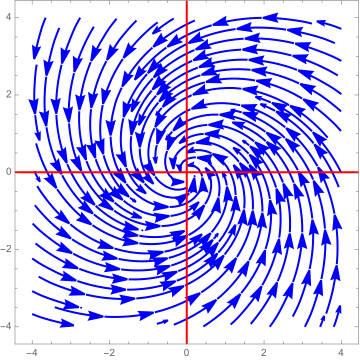
\includegraphics[width=0.4\textwidth]{additional/Stability/Points/StableFocal.pdf}
					\caption{Устойчивый фокус}
					\label{Stability:StableFocal}
				\end{figure}

			\columnbreak

				\begin{figure}[H]
					\centering
					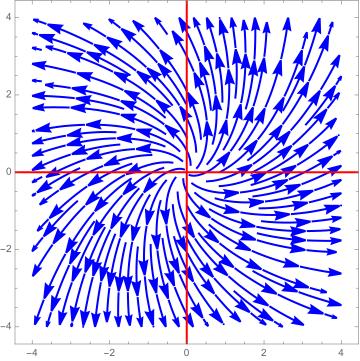
\includegraphics[width=0.4\textwidth]{additional/Stability/Points/UnstableFocal.pdf}
					\caption{Неустойчивый фокус}
					\label{Stability:UnstableFocal}
				\end{figure}

			\end{multicols}

		\item \textit{Центр} -- случай, когда комплексно-сопряженные собственные значения $\lambda_{1, 2}$ имеют нулевую вещественную часть (положим $\lambda_{1, 2} = \pm i \beta, ~ \beta \in \mathbb{R}, ~ \lambda_{1, 2} \in \mathbb{C}$). Интегральные кривые представляют собой семейство эллипсов, окружающих точку покоя. Вращение производится в положительном направлении вращения системы координат (по часовой стрелке) в случае, если вещественная жорданова форма является обобщением комплексного числа. На изображении ниже рассмотрен случай $J = \begin{pmatrix} 0 & -1 \\ 1 & 0 \end{pmatrix}$ (устойчивый фокус, рис. \ref{Stability:Circular}). 

			\begin{figure}[H]
				\centering
				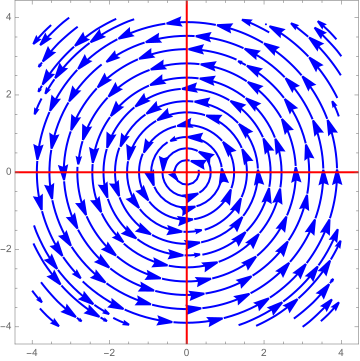
\includegraphics[width=0.4\textwidth]{additional/Stability/Points/Circular.pdf}
				\caption{Центр}
				\label{Stability:Circular}
			\end{figure}

		\item \textit{Семейство параллельных прямых} -- случай, когда среди вещественных собственных значений $\lambda_{1, 2}$ имеется хотя-бы одно отрицательное собственное значение (положим $\lambda_1 = 0, \lambda_2 \neq 0, ~ \lambda_{1, 2} \in \mathbb{R}$). В случае, если хотя бы одно из собственных значений не нулевое, интегральные кривые представляют собой параллельные прямые, параллельные прямой, образованной собственным вектором, отвечающим ненулевому собственному значению, и сходящиеся к (в случае одного отрицательного собственного значения), или исходящие из (в случае одного положительного собственного значения) прямой, образованной собственным вектором, отвечающим за нулевое собственное значение. На изображениях ниже рассмотрены случаи $J = \begin{pmatrix} -2 & 0 \\ 0 & 0 \end{pmatrix}$ (устойчивое семейство параллельных прямых, рис. \ref{Stability:StableParallel}) и $J = \begin{pmatrix} 1 & 0 \\ 0 & 0 \end{pmatrix}$ (неустойчивое семейство параллельных прямых, рис. \ref{Stability:UnstableParallel}).

			\begin{multicols}{2}

				\begin{figure}[H]
					\centering
					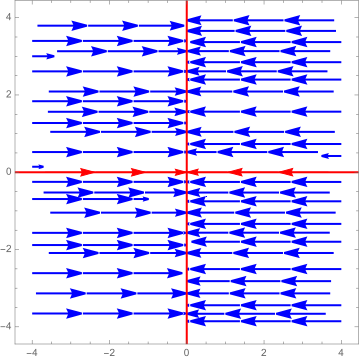
\includegraphics[width=0.35\textwidth]{additional/Stability/Points/StableParallel.pdf}
					\caption{Сходящееся семейство параллельных прямых}
					\label{Stability:StableParallel}
				\end{figure}

			\columnbreak

				\begin{figure}[H]
					\centering
					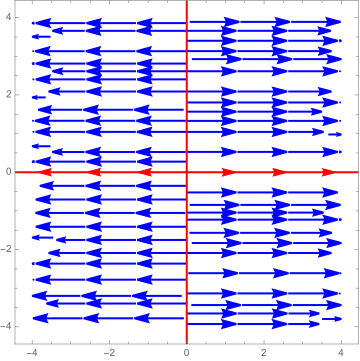
\includegraphics[width=0.35\textwidth]{additional/Stability/Points/UnstableParallel.pdf}
					\caption{Расходящееся семейство параллельных прямых}
					\label{Stability:UnstableParallel}
				\end{figure}

			\end{multicols}

			В случае, если оба собственных значения нулевые, и линейно-зависимы (положим $\lambda_1 = \lambda_2 = 0$), то параллельные прямые разнонаправлены. Выше прямой, образованной первым направляющим вектором параллельные прямые направлены в сторону его положительного направления, ниже -- отрицательного. В случае, когда нулевые значения линейно-независимы, фазовое пространство находится в покое. На изображении ниже рассмотрен случай $J = \begin{pmatrix} 0 & 1 \\ 0 & 0 \end{pmatrix}$ (неустойчивое семейство параллельных разнонаправленных прямых, рис. \ref{Stability:UnstableLinearFlow})
			
			\begin{figure}[H]
				\centering
				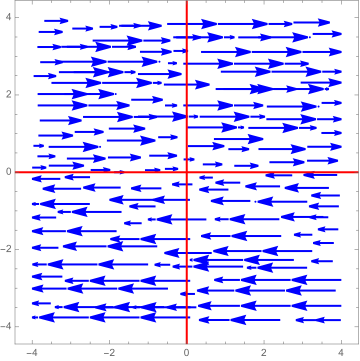
\includegraphics[width=0.5\textwidth]{additional/Stability/Points/UnstableLinearFlow.pdf}
				\caption{Неустойчивое семейство параллельных разнонаправленных прямых}
				\label{Stability:UnstableLinearFlow}
			\end{figure}

	\end{enumerate}


	\subsection{Примеры}

		В качестве примера рассмотрим следующую систему нелинейных дифференциальных уравнений:
		\[ \syst{\dot{x} &= y \cos{x}, \\ \dot{y} &= \sin{x}.} \]
		Найдем ее стационарные точки. Для это построим решение следующей системы:
		\[ \syst{&y \cos{x} = 0 \\ &\sin{x} = 0} \implies \syst{x &= \pi k, ~ k \in \mathbb{Z}, \\ y &= 0.} \]
		Построим соответствующую линеаризованную систему в окрестности точек $M_k = \pares{\pi k, 0}$:
		\[ 
			\tilde{J} \pares{x, y} \sat_{x = \pi k, ~ y = 0} = 
			\begin{pmatrix}
				-y \sin{x} & \cos{x} \\ \cos{x} & 0
			\end{pmatrix} \sat_{x = \pi k, ~ y = 0} = 
			\begin{pmatrix}
				0 & (-1)^k \\ (-1)^k & 0
			\end{pmatrix}
		\]
		Собственные значения матрицы: $\lambda_{1, 2} = \pm 1$ -- вещественные, разных знаков, соответственно точки $M_k = \pares{\pi k, 0}$ являются седловыми. Собственные вектора матрицы:
		\[ \lambda_1 = -1: \vec{v}_1 = \begin{pmatrix} (-1)^k \\ -1 \end{pmatrix}, ~ \lambda_2 = 1: \vec{v}_2 = \begin{pmatrix} (-1)^k \\ 1 \end{pmatrix}. \]
		Матрица преобразования, и жорданова форма имеют следующий вид:
		\[ P = \begin{pmatrix} (-1)^k & (-1)^k \\ -1 & 1 \end{pmatrix}, ~ J = \begin{pmatrix} -1 & 0 \\ 0 & 1 \end{pmatrix}. \]
		Применим преобразование $P$ для фазового пространства, описанного на рис. (\ref{Stability:Saddle}):
		\begin{multicols}{2}

			\begin{figure}[H]
				\centering
				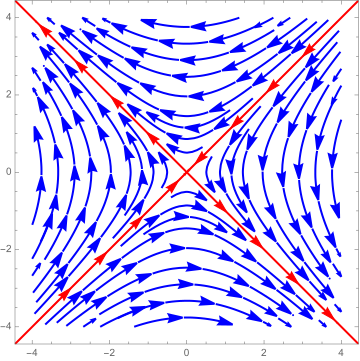
\includegraphics[width=0.35\textwidth]{additional/Stability/Points/Example1Odd.pdf}
				\caption{Седловая точка в случае $k$ -- нечетных}
				\label{Stability:Example1Odd}
			\end{figure}

		\columnbreak

			\begin{figure}[H]
				\centering
				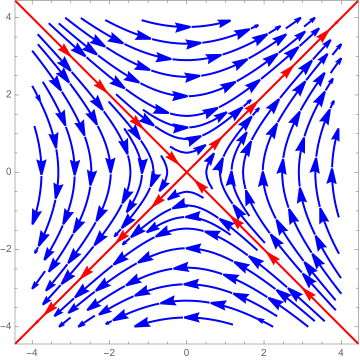
\includegraphics[width=0.35\textwidth]{additional/Stability/Points/Example1Even.pdf}
				\caption{Седловая точка в случае $k$ -- четных}
				\label{Stability:Example1Even}
			\end{figure}

		\end{multicols}
		Объединим данные траектории на общем изображении:
		\begin{figure}[H]
			\centering
			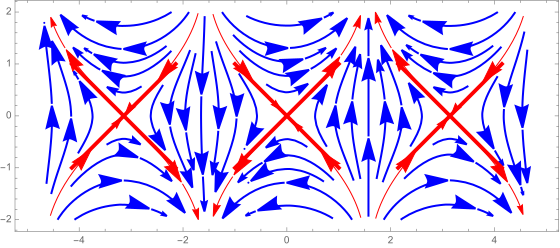
\includegraphics[width=0.7\textwidth]{additional/Stability/Points/Example1Sol.pdf}
			\caption{Фазовое пространство решения}
			\label{Stability:Example1Sol}
		\end{figure}

		Рассмотрим следующий пример:
		\[ \left\lbrace \begin{split}
			\dot{x} &= - 2 x^2 y - 2 x y^2 - 2 y^2 + 22 y \\
			\dot{y} &= 2 x^2 y - 2 x y + 2 y^2 - 22 y
		\end{split} \right. \]
		Найдем нули системы:
		\[ 
			\syst{
				&y \pares{x^2 + xy + y - 11} = 0 \\ &y \pares{x^2 - x + y - 11} = 0 
			} \implies \begin{split} 
				&M_0 = \pares{C, 0}, ~ M_1 = \pares{0, 11}, \\ 
				&M_2 = \pares{-3, -1}, ~ M_3 = \pares{4, -1}. 
			\end{split} 
		\]
		Матрица Якоби исходной системы имеет следующий вид: 
		\[
			\tilde{J} = \begin{pmatrix}
				- 4xy - 2y^2 & - 2 x^2 - 4xy - 4y + 22 \\ 
				4xy - 2y & 2 x^2 - 2x + 4y - 22
			\end{pmatrix}
		\]

		Рассмотрим точку $M_0$. Матрица Якоби в окрестности точки $M_0$ принимает вид:
		\[
			\tilde{J} = \begin{pmatrix}
				0 & 22 - 2C^2 \\
				0 & -22 + 2C^2
			\end{pmatrix}
		\]
		Собственные значения и соответствующие им собственные вектора следующие:
		\[ \lambda_1 = 0: \vec{v}_1 = \begin{pmatrix} 1 \\ 0 \end{pmatrix}, ~ \lambda_2 = -22 + 2C^2: \vec{v}_2 = \begin{pmatrix} 1 \\ -1 \end{pmatrix}. \]
		Так как среди собственных значений присутствует хотя-бы один ноль, то точка $M_0 \forall C$ является семейством параллельных прямых. В случае, если $C^2 < 11$ -- интегральные прямые сходятся к прямой, образованной вектором $\vec{v}_1$ перпендикулярно вектору $\vec{v}_2$; если $C^2 > 11$ -- интегральные прямые исходят из прямой, образованной вектором $\vec{v}_1$ перпендикулярно вектору $\vec{v}_2$; если $C^2 = 11$, то окрестность находится в состоянии покоя.

		Рассмотрим точку $M_1$. Матрица Якоби в окрестности точки $M_1$ принимает вид:
		\[
			\tilde{J} = \begin{pmatrix}
				-242 & -22 \\
				-22 & 22
			\end{pmatrix}
		\]
		Собственные значения и соответствующие им собственные вектора следующие:
		\[ \lambda_{1, 2} = 22 \pares{-5 \pm \sqrt{37}}: \vec{v}_{1, 2} = \begin{pmatrix} 6 \pm \sqrt{37} \\ 1 \end{pmatrix}. \]
		Собственные значения разных знаков, тогда точка $M_1$ -- неустойчивая седловая точка. Интегральные кривые сходятся вдоль прямой, образованной вектором $\vec{v}_2$, и расходятся вдоль прямой, образованной вектором $\vec{v}_1$.

		Рассмотрим точку $M_2$. Матрица Якоби в окрестности точки $M_2$ принимает вид:
		\[
			\tilde{J} = \begin{pmatrix}
				-14 & -4 \\
				14 & -2
			\end{pmatrix}
		\]
		Собственные значения и соответствующие им собственные вектора следующие:
		\[ \lambda_{1, 2} = -8 \pm i \cdot 2\sqrt{5}: \vec{v}_{1, 2} = \begin{pmatrix} -3 \pm i \sqrt{5} \\ 7 \end{pmatrix}. \]
		Оба собственных значения комплексные, с отрицательной вещественной частью, тогда точка $M_2$ -- устойчивый фокус. Вещественная матрица преобразования и матрица комплексного числа примут следующий вид:
		\[ P = \begin{pmatrix} 2 & -2 \\ \sqrt{5} - 3 & \sqrt{5} + 3 \end{pmatrix}, ~ J = \begin{pmatrix} -8 & -2\sqrt{5} \\ 2\sqrt{5} & -8 \end{pmatrix}. \]

		Рассмотрим точку $M_3$. Матрица Якоби в окрестности точки $M_3$ принимает вид:
		\[
			\tilde{J} = \begin{pmatrix}
				14 & 10 \\
				-14 & -2
			\end{pmatrix}
		\]
		Собственные значения и соответствующие им собственные вектора следующие:
		\[ \lambda_{1, 2} = 6 \pm i \cdot 2\sqrt{19}: \vec{v}_{1, 2} = \begin{pmatrix} 4 \pm i \sqrt{19} \\ -7 \end{pmatrix}. \]
		Оба собственных значения комплексные, с положительной вещественной частью, тогда точка $M_2$ -- неустойчивый фокус. Вещественная матрица преобразования и матрица комплексного числа примут следующий вид:
		\[ P = \begin{pmatrix} -5 & 5 \\ \sqrt{19} + 4 & \sqrt{19} - 4 \end{pmatrix}, ~ J = \begin{pmatrix} 6 & -2\sqrt{19} \\ 2\sqrt{19} & 6 \end{pmatrix}. \]

		Объединим все точки и траектории в их окрестности на общем изображении:
		\begin{figure}[H]
			\centering
			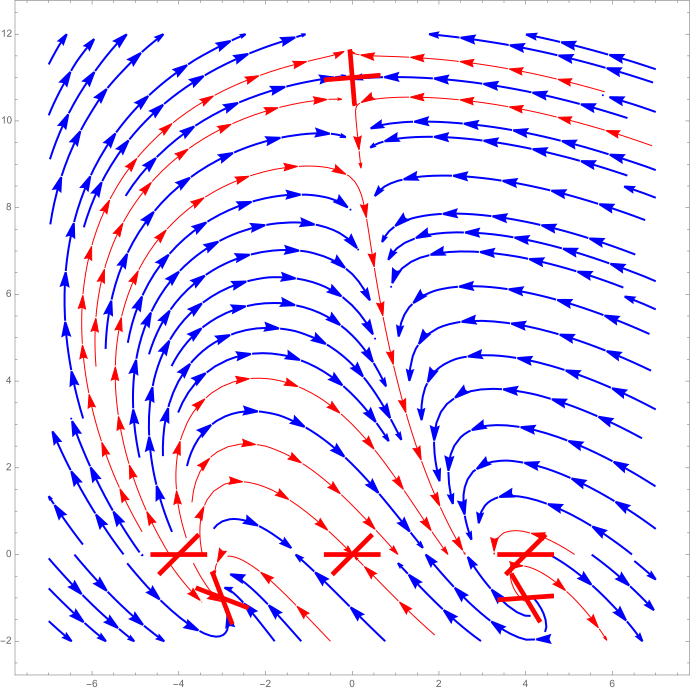
\includegraphics[width=0.7\textwidth]{additional/Stability/Points/Example2Sol.pdf}
			\caption{Фазовое пространство решения}
			\label{Stability:Example2Sol}
		\end{figure}

	% \pagebreak